\subsection{Working of LIGO}

\subsubsection{Working of laser system}

To operate LIGO at its fullest potential, we need an immensely powerful laser. In order to obtain such a laser beam, it must undergo multiple stages of amplification. Initially Nd-YAG laser produces a beam in the near-infrared region of the electromagnetic spectrum at 1064 $nm$. then the beam passes through Non-Planar Ring Oscillator (NPRO), Master-Oscillator Power Amplifier (MOPA) which consists of four thin rods and finally through High-Power Oscillator (HPO). Thus a powerful laser of power $200\,W$, with wavelength $1064\,nm$ is obtained. 

\subsubsection{Working of Fabry-Perot cavity and Beam splitter}

Then the powerful collimated light beam incidents on a power recycling mirror followed by a beam splitter. The partially reflecting beam splitter splits the light into the $4\,km$ long ultra-high vacuum chambers which are present orthogonal to each other. The laser beam is spread to a diameter of 6cm when it reaches each mirror reducing the thermal effects of heating the mirror surface. The Fabry-Perot cavities make the light to reflect $\approx 300$ times which increases the laser power to $100\,kW$. Thus as the laser accumulates power gradually, after a certain value the beam splitter allows the laser beam to pass through it towards the photo-detector. The interferometer is designed such that these two coherent light beams from the perpendicular arms recombine at the beam splitter almost exactly out of phase thereby mostly cancelling the output signal when the two arms are of the same length, and the photo detector shouldn't receive any light if no disturbances are present. However, this is not the scenario if a gravitational wave passes nearby. \cite{Interferometer}

\begin{figure}[h]
    \centering
    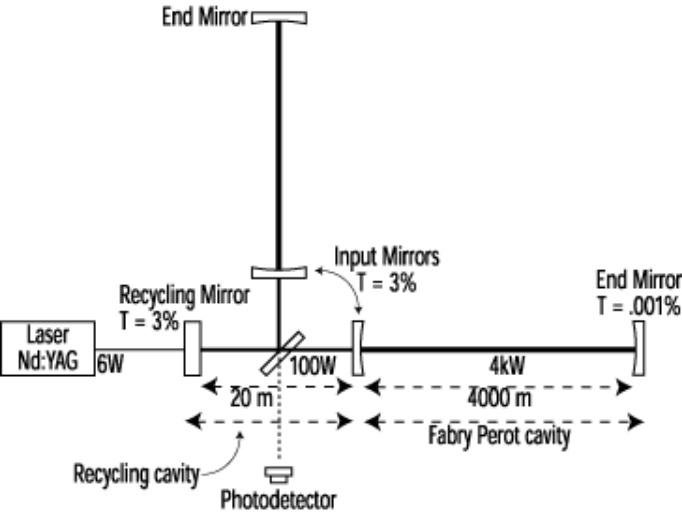
\includegraphics[scale=0.7]{images.tex/Working of Fabry-Perot cavity.jpg}
    \caption{Working of Fabry-Perot cavity. Source :- \href{https://spie.org/news/ligo-researchers-design-complex-device-to-detect-infinitesimal-changes?SSO=1}{spie.org}}
\end{figure}

\subsubsection{Working of Interferometer when gravitational wave passes}

As we saw the effect of gravitational waves, which stretch the space in one direction and compress it in the perpendicular direction. Hence, when the gravitational wave passes through the arms of LIGO, they will be subjected to compressing and stretching strain, so if the length of one arm increases, simultaneously length of other arm decreases. Even the laser light get compressed and stretched which alters the phase difference between the perpendicular light beams which causes a variation in the effective length travelled by the laser beam. Hence when the light recombine neither destructively nor constructively, where the resultant amplitude decides the intensity (I) of light that will be detected finally according to the relation

\begin{equation}
     I \propto (A_1)^2 + (A_2)^2 + 2(A_1)(A_2)\text{cos}(\Delta \phi)
\end{equation}

where $A_1$ and $A_2$ are the amplitudes of laser from LIGO's arms and $\Delta \phi$ is the phase difference between the interfering light beams. 

\begin{figure}[h]
    \centering
    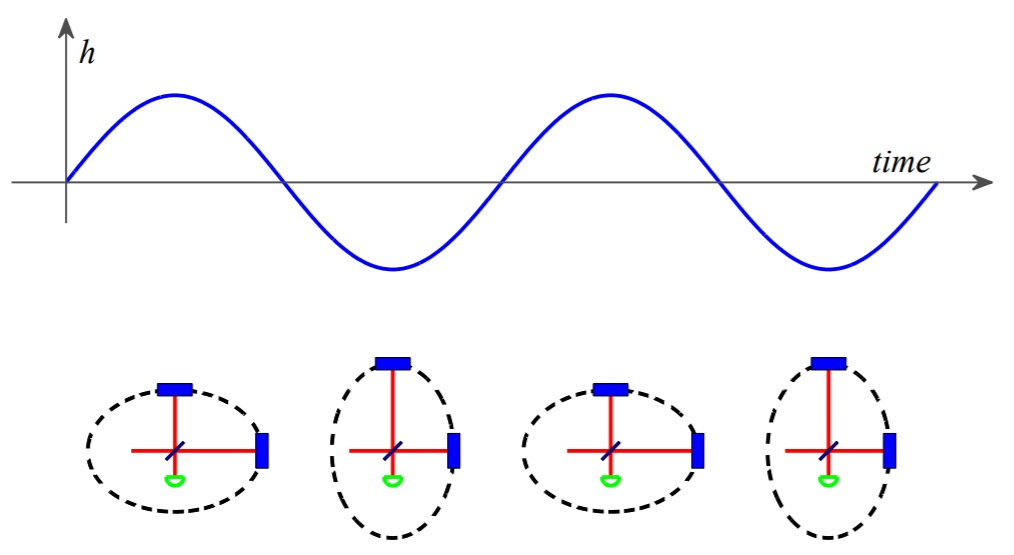
\includegraphics[scale =0.6]{images.tex/GW effect on LIGO arm.jpg}
    \caption{Gravitational wave effect on LIGO arms. Source :- \href{https://www.semanticscholar.org/paper/Broadband-Measurement-and-Reduction-of-Quantum-in-Cripe/ffe14b1a34d504599fa81c817bbb9aef5385c06c}{Semanticscholar.org} \cite{Cripe2020BroadbandMA}}
\end{figure}

So if there is no disturbance, then the arms will be intact, thus the light interfere destructively and the intensity of light detected by the photo detector will be zero, thus no signal is recorded. But if gravitational wave passes, due to change in length of LIGO arms, a phase difference will be created such that the light will interfere partially, thus the intensity of light will fluctuate. The frequency of fluctuation of intensity will be a function of time which will be calculated by the photo detector and that can be converted to the strain caused on the arms which in turn will be a function of frequency. This will be calculated by the computers which is generally shown as the wave form of the detected gravitational wave. 

\begin{figure}[h]
    \centering
    \subfloat[]{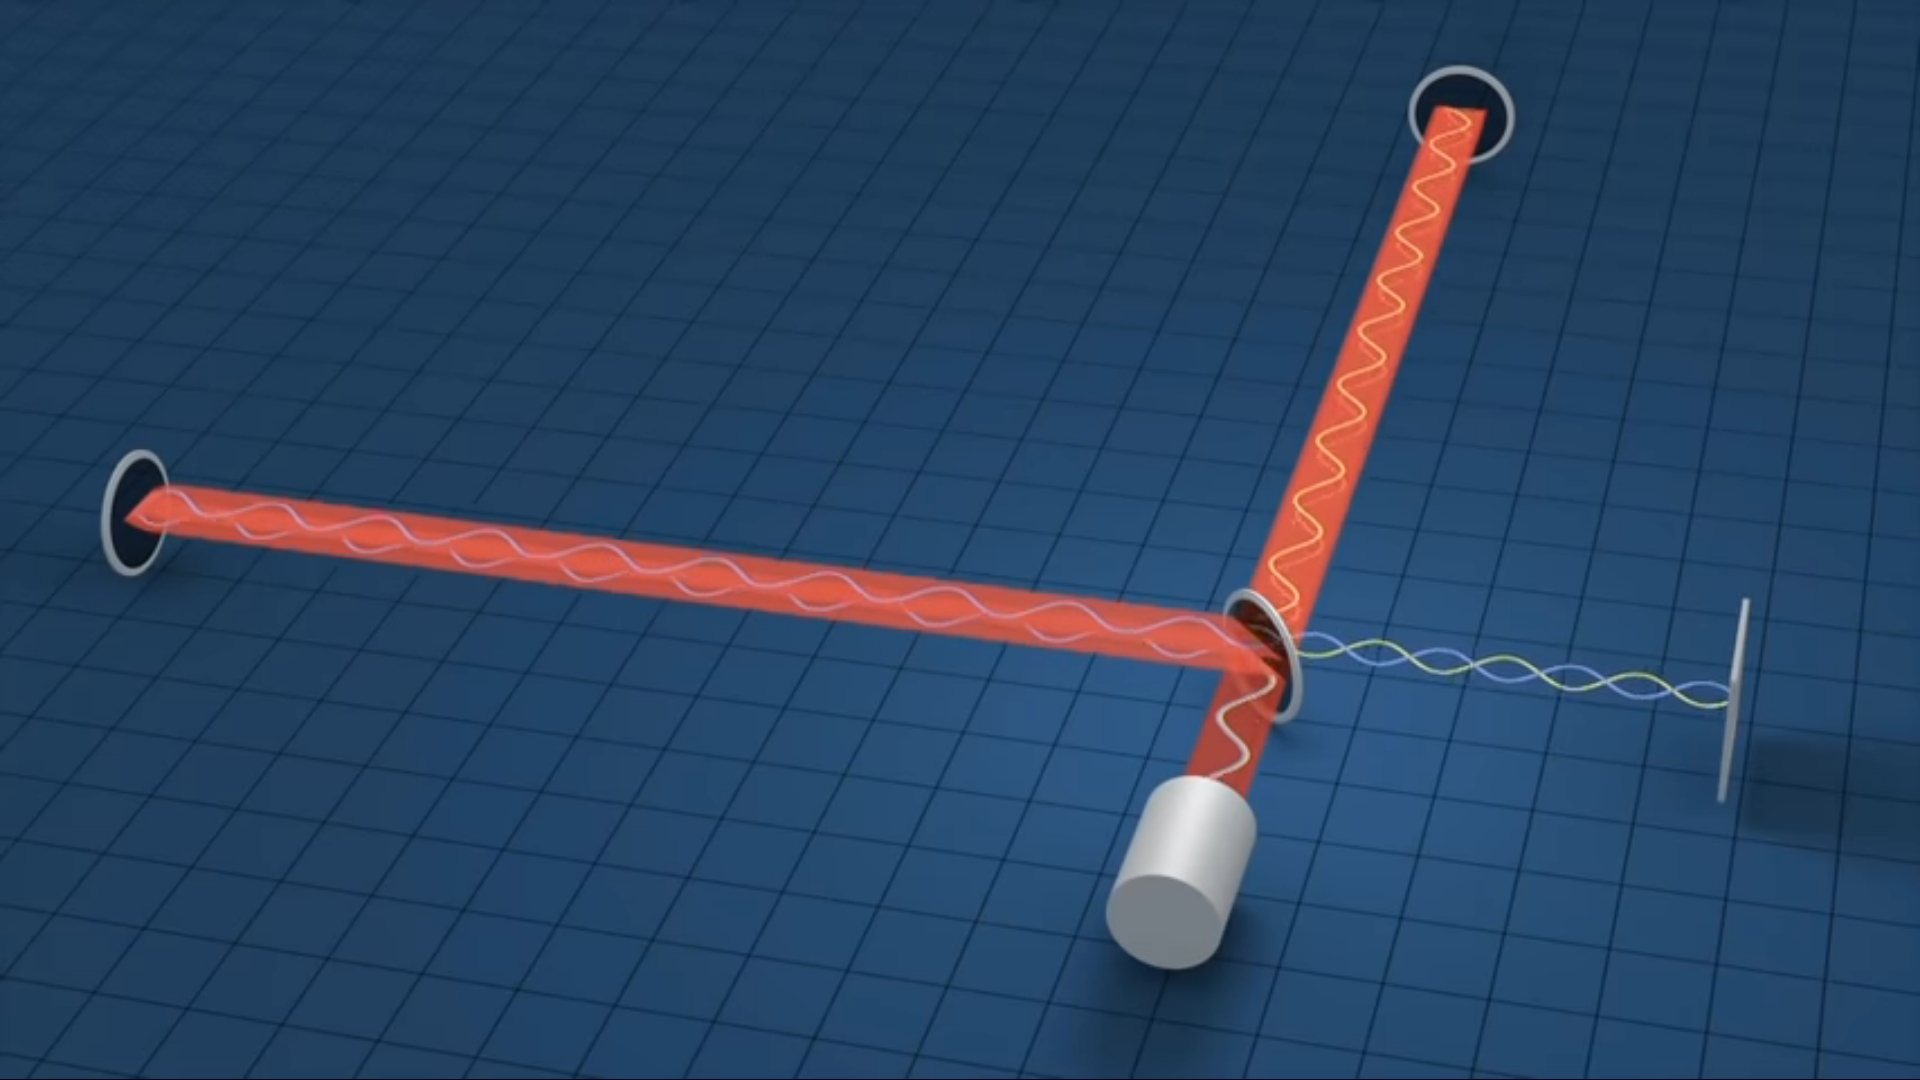
\includegraphics[width = 5.5 cm, height = 4 cm]{images.tex/Initial condition.png}}
    \qquad
    \subfloat[]{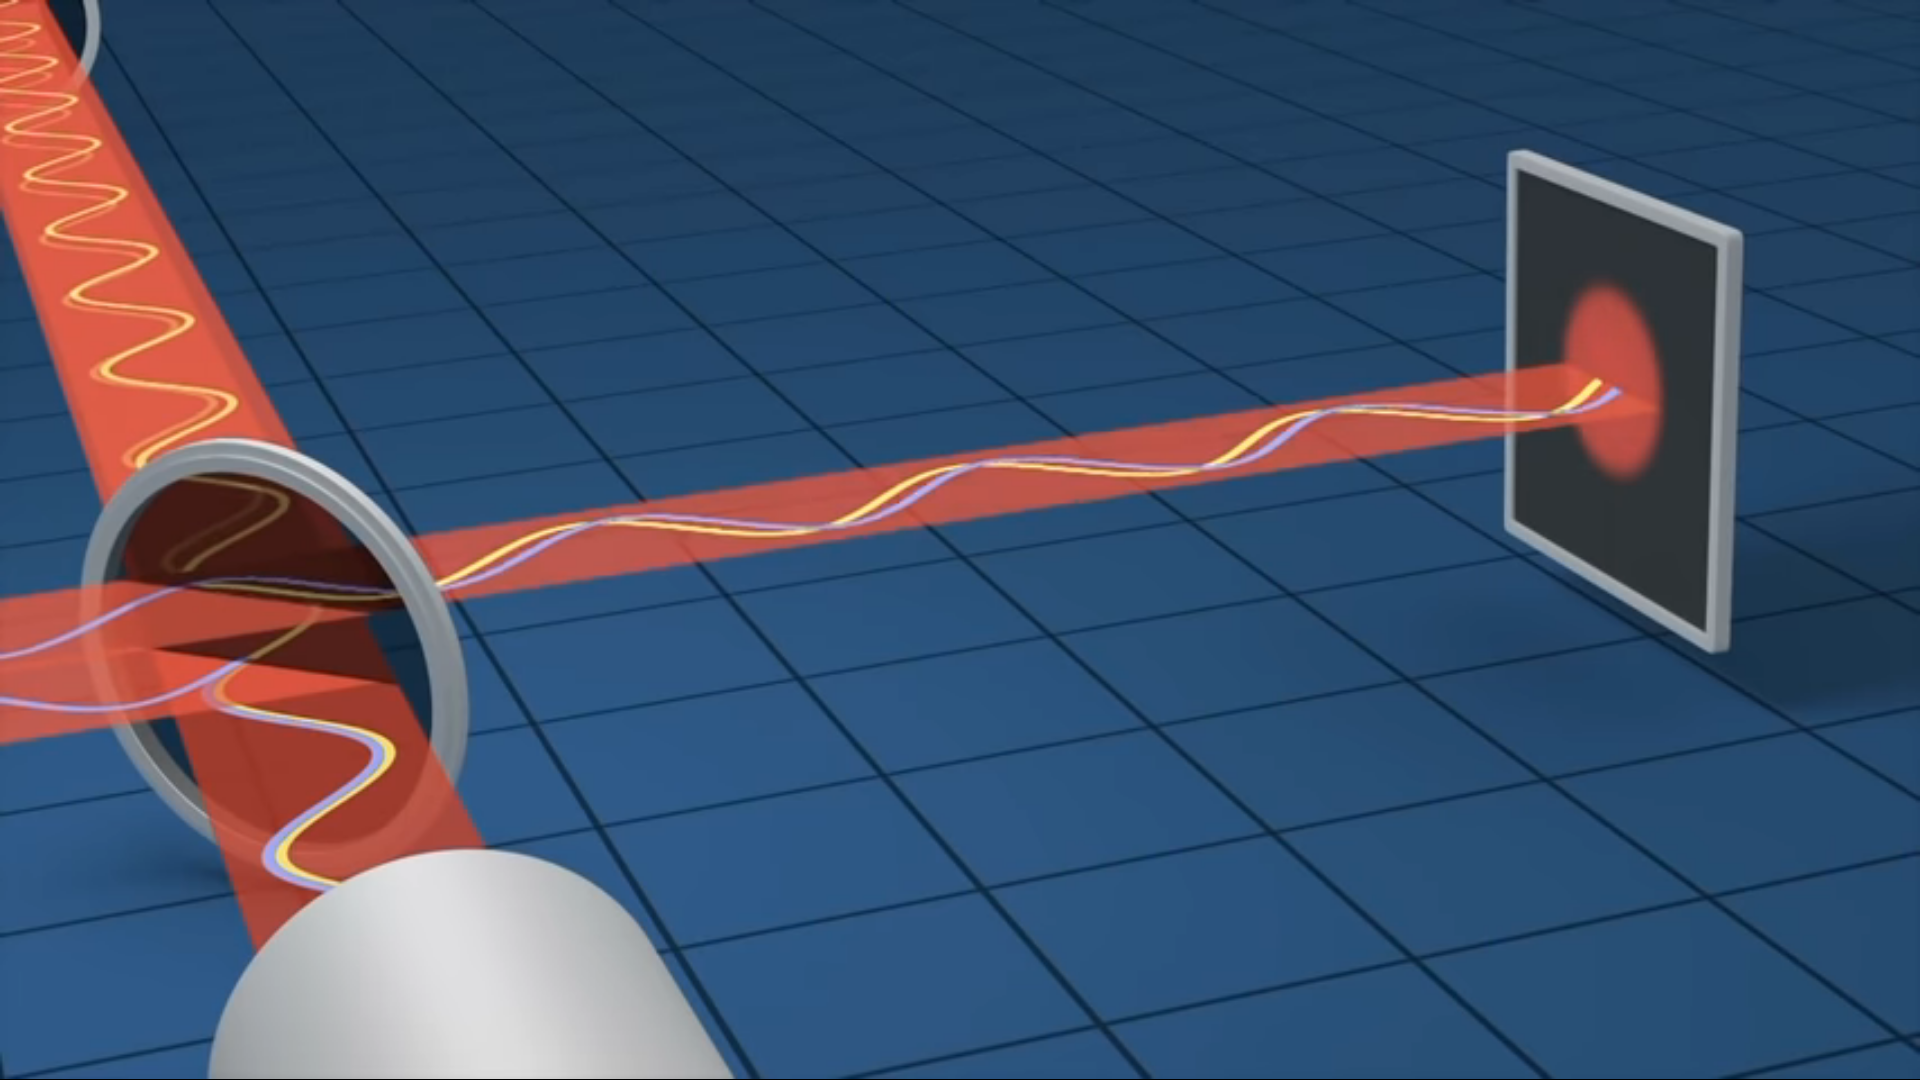
\includegraphics[width = 5.5 cm, height = 4 cm]{images.tex/Constructive.png}}
    \qquad
    \subfloat[]{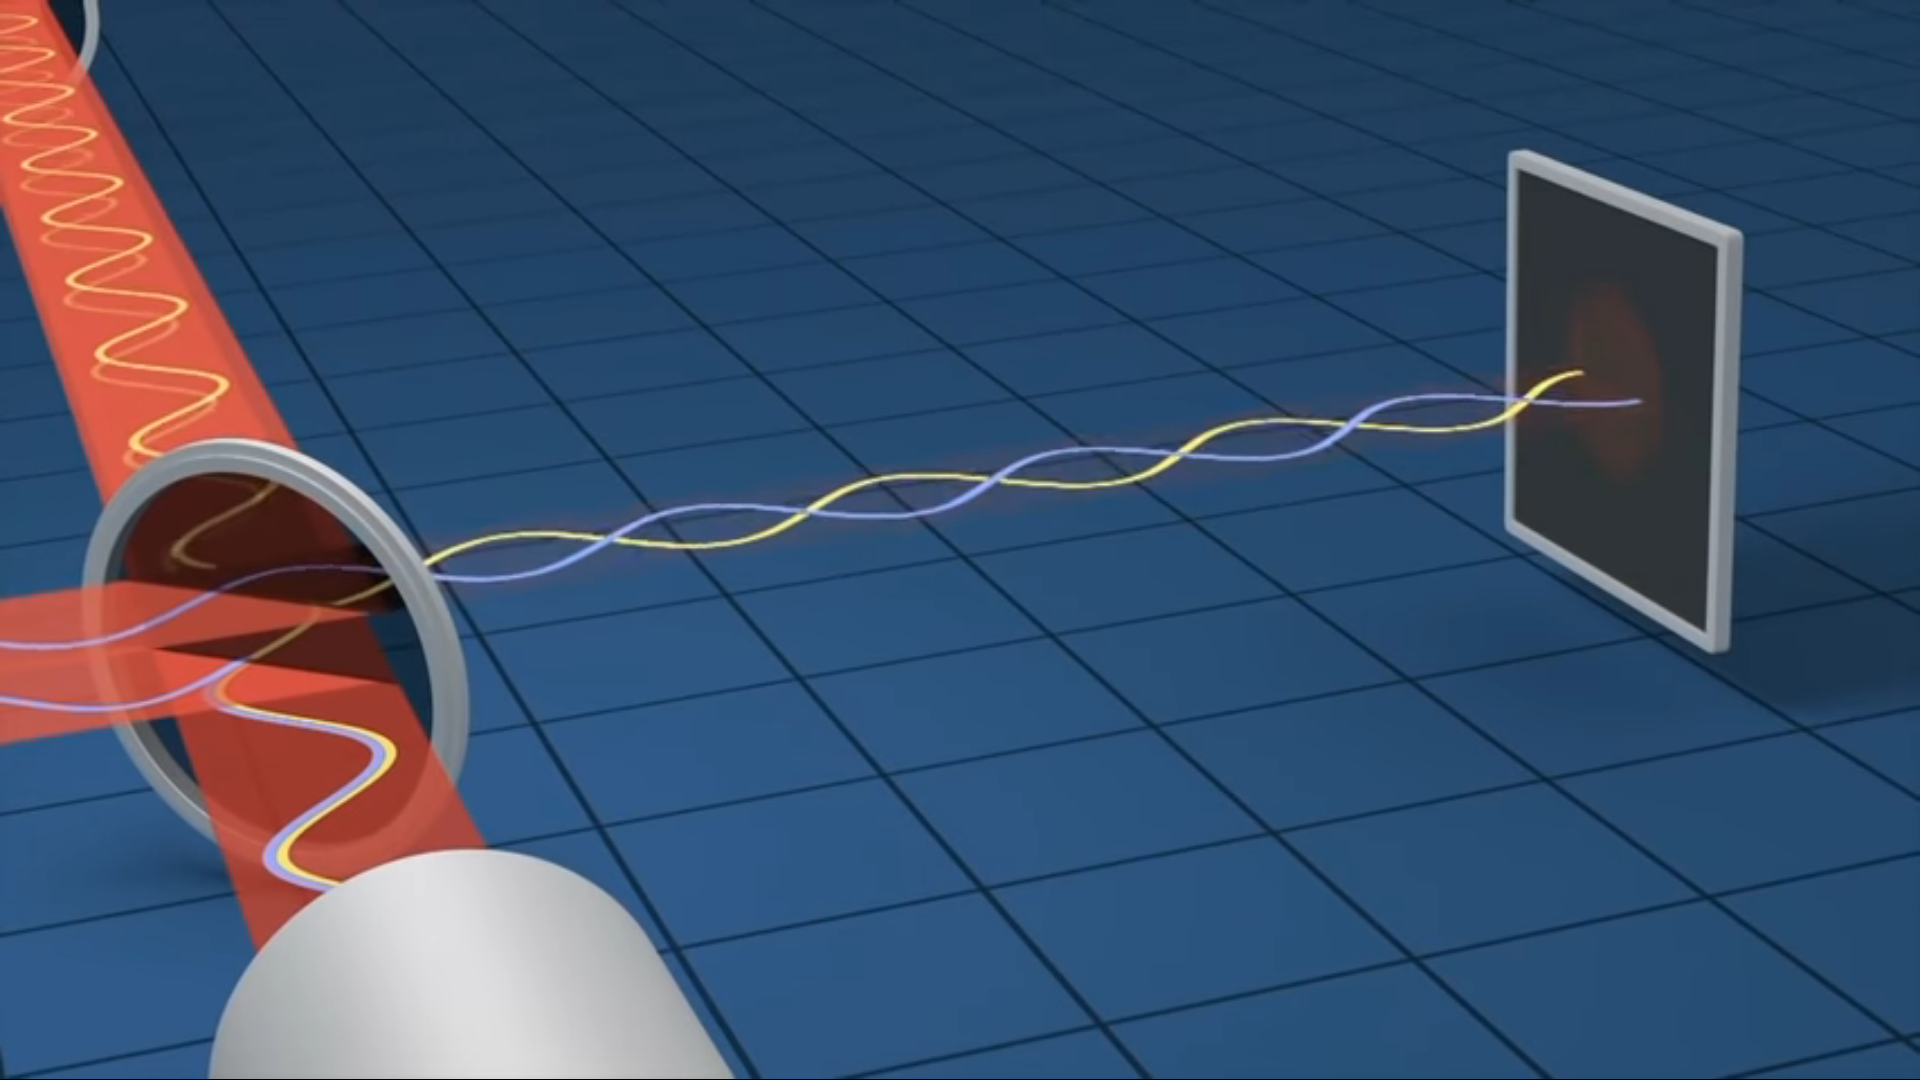
\includegraphics[width = 5.5 cm, height = 4 cm]{images.tex/Destructive.png}}
    \qquad
    \subfloat[]{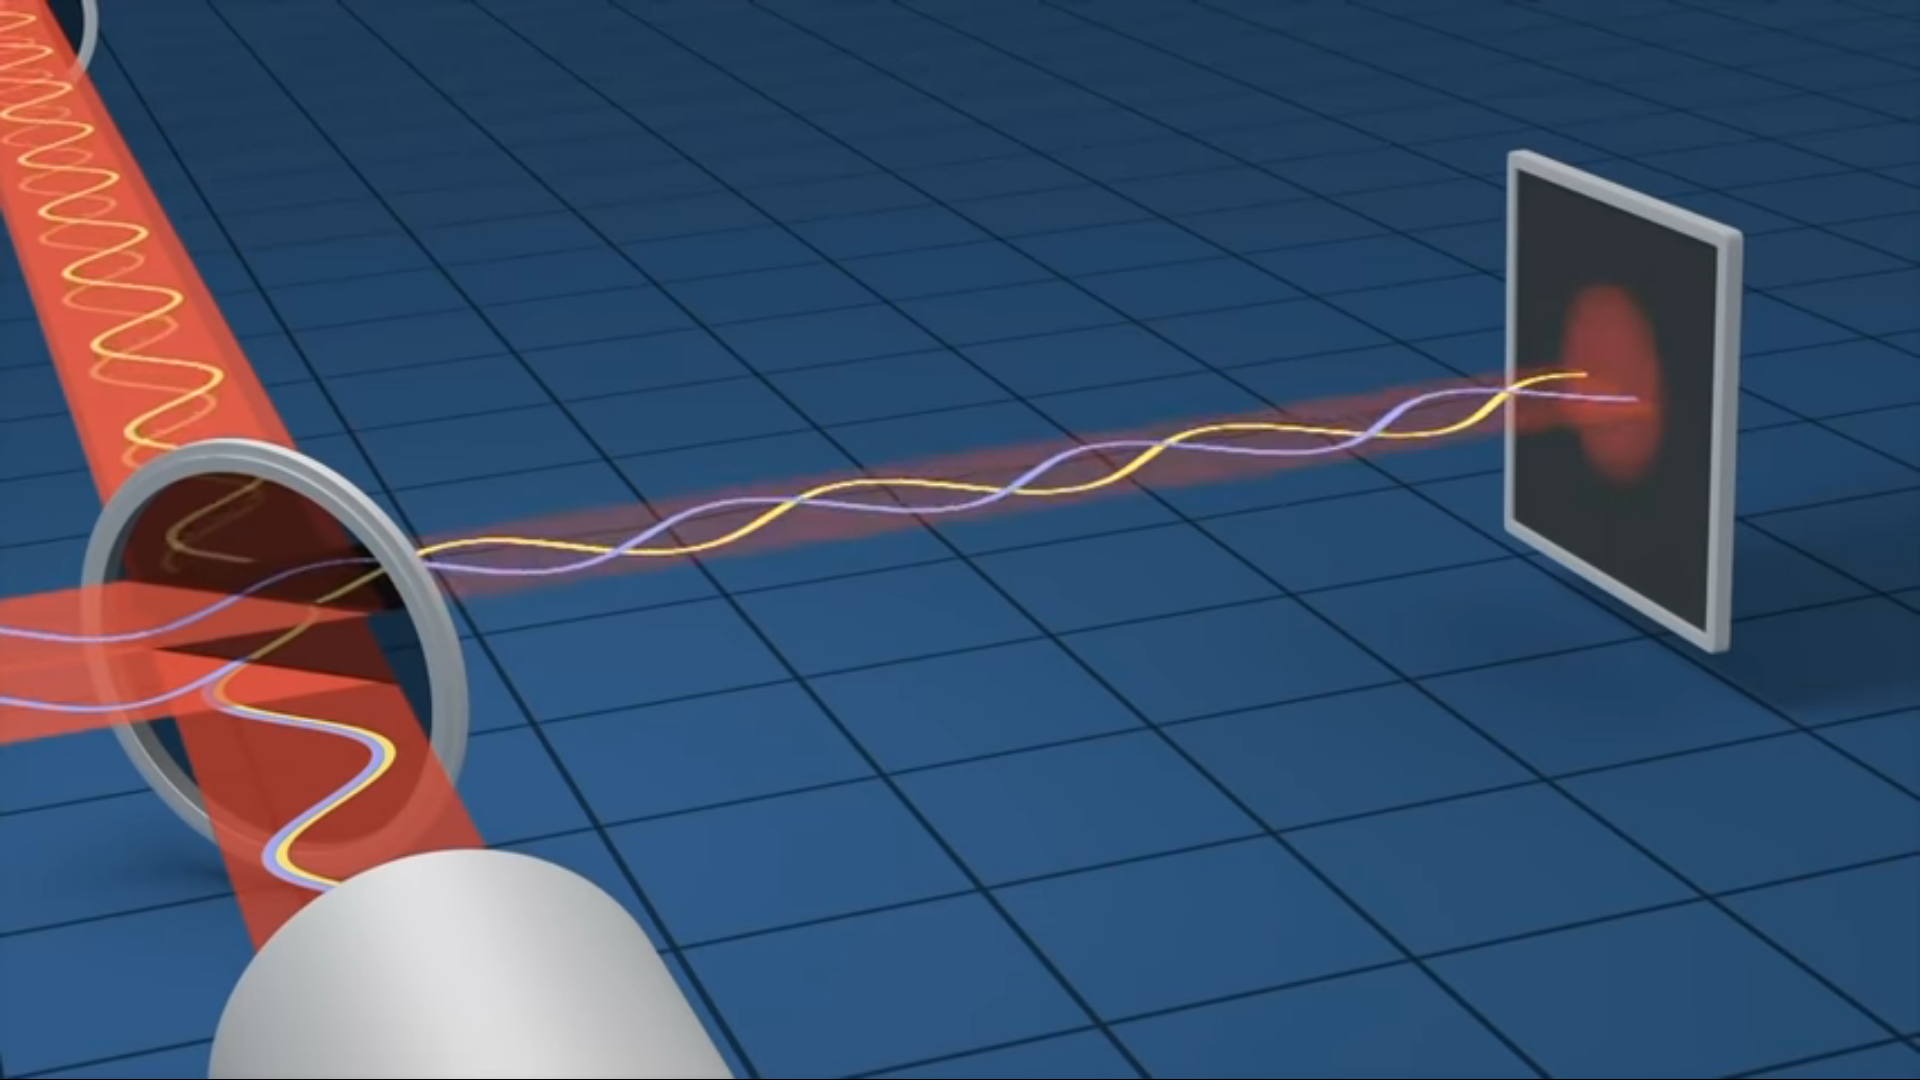
\includegraphics[width = 5.5 cm, height = 4 cm]{images.tex/Intermediate.png}}
    \caption{(a) Initial Condition (b) Constructive interference.\\
    (c) Destructive interference (d) Partial interference}
\end{figure}

But apart from gravitational waves, there are other disturbances also. Like earthquakes which can also influence the interference pattern. To avoid this as much, the whole system is evacuated. Other measures are also taken to dampen these vibrations which are described in noise cancellation.

\pagebreak















































































\pagebreak
